\documentclass[a4paper, 12pt,titlepage,openany]{report}

\usepackage[british]{babel}

\usepackage[T1]{fontenc}
\usepackage[utf8]{inputenc}

\usepackage{lipsum}

\usepackage[hidelinks]{hyperref}
\hypersetup{pdfauthor={Edmund Jochim, Axit Kakadiya, Devraj Solanki, Anil Chhotala}, 
	pdftitle={Design and Development for the Control of a Mecanum Wheel Car},
	pdfkeywords={Mecanum Wheel, ESP32},
	pdfcreationdate=2024,
	colorlinks=false,
	linkbordercolor={1 1 1},
	citebordercolor={1 1 1},
	urlbordercolor={1 1 1}
}

\usepackage{xcolor} % For custom colors

\usepackage{parskip}

\usepackage{caption}

\usepackage{subcaption}

\usepackage{listings}


% Define custom colors
\definecolor{codeblue}{rgb}{0.2,0.2,0.8}
\definecolor{codegreen}{rgb}{0.0,0.6,0.0}
\definecolor{codegray}{rgb}{0.5,0.5,0.5}
\definecolor{codepurple}{rgb}{0.58,0.0,0.82}
\definecolor{backcolor}{rgb}{0.95,0.95,0.92}

% Configure the listings package for C++
\lstdefinestyle{customcpp}{
	language=C++, % Specify language
	frame=tb, % Draw top and bottom frame lines
	aboveskip=3mm,
	belowskip=3mm,
	showstringspaces=false, % Do not show spaces in strings as underscores
	columns=flexible,
	keepspaces=true,
	basicstyle={\small\ttfamily}, % Set font style
	numbers=left, % Line numbers on the left
	numberstyle=\tiny\color{codegray}, % Style for line numbers
	keywordstyle=\color{codeblue}, % Keywords in blue
	commentstyle=\color{codegreen}, % Comments in green
	stringstyle=\color{codepurple}, % Strings in purple
	backgroundcolor=\color{backcolor}, % Background color for code block
	breaklines=true, % Allow line breaks in code
	breakatwhitespace=true, % Break lines at whitespaces if needed
	tabsize=4, % Set tab size
	captionpos=b, % Caption position at the bottom
	escapeinside={\%*}{*)}, % If you need to escape to LaTeX inside code
	morekeywords={define, uint8\_t, int8\_t, int16\_t, IPAddress}, % Add additional keywords
}

\usepackage[a4paper,
left=2.5cm,
right=2cm,
top=2cm,
bottom=2cm,
ignorefoot=false]
{geometry}

\usepackage{amsmath}
\usepackage{amsfonts}
\usepackage{amssymb}
\usepackage{algorithmic}

\usepackage{siunitx}

\usepackage{cite}

\usepackage{graphicx}

\usepackage{fancyhdr}

\usepackage[printonlyused]{acronym}

\usepackage{tcolorbox}
\usepackage{makecell}
\usepackage{tabularx}

\usepackage{todonotes}

\addto{\captionsbritish}{\renewcommand{\bibname}{References}}
\addto{\captionsbritish}{\renewcommand{\contentsname}{Table of Contents}}

\graphicspath{{./graphic/}}

\hbadness 100000
\sloppy
\frenchspacing

\usepackage{array}
\newcolumntype{L}[1]{>{\raggedright\let\newline\\\arraybackslash\hspace{0pt}}m{#1}}
\newcolumntype{C}[1]{>{\centering\let\newline\\\arraybackslash\hspace{0pt}}m{#1}}
\newcolumntype{R}[1]{>{\raggedleft\let\newline\\\arraybackslash\hspace{0pt}}m{#1}}

\usepackage{titlesec}
\titleformat{\chapter}{\bfseries\Large}{\arabic{chapter}.~}{0pt}{}

\renewcommand*{\familydefault}{\sfdefault}
\usepackage[scaled]{helvet}

\setlength{\parindent}{0pt}

\setlength{\parskip}{1.5ex plus 0.5ex minus 0.5ex}

\renewcommand{\baselinestretch}{1.15}


\bibliographystyle{IEEEtran}

\begin{document}
	\pagenumbering{Roman}
	\thispagestyle{empty}
	
	\begin{flushleft}
		\begin{figure}[!htb]
			\centering
			\vspace*{-1\baselineskip}
			
\includegraphics[scale=.45]{Logo_THM_CF_FB11_4c.eps}
		\end{figure}
	\end{flushleft}
	\vspace*{3\baselineskip}
	\begin{center}
		CCCE\\
		\textbf{Case Study Project}\\
		Summer Semester 2024
		\vspace*{3\baselineskip}
		\hrule
		\vspace*{1\baselineskip}
		{\LARGE \textbf{Design and Development for the\\Control of a Mecanum Wheel Car}}
		\vspace*{1.3\baselineskip}
		\hrule
		\vspace*{2\baselineskip}
		Anil Manubhai Chhotala\\
		Matriculation Number: ...\\
		\vspace*{1\baselineskip}
		Axit Kantibhai Kakadiya\\
		Matriculation Number: ...\\
		\vspace*{1\baselineskip}
		Devraj Ajaykumar Solanki\\
		Matriculation Number: ...\\
		\vspace*{1\baselineskip}
		Edmund Jochim\\
		Matriculation Number: 5729098\\
		\vspace*{3\baselineskip}
		\begin{tabular}{lcl}
			Supervisor: &  & Prof. Dr.-Ing. Fabian Mink\\
			& &\\
			Submitted on: & & xx.09.2024
		\end{tabular}
	\end{center}
	
	\clearpage
	\renewcommand{\baselinestretch}{1.15}
	\normalsize
	
	\begin{abstract}
		\thispagestyle{plain}
		\setcounter{page}{2}
		
	\end{abstract}
	
	\cleardoublepage
	\setcounter{page}{3}
	
	\tableofcontents
	
	\chapter*{Declaration of Authorship}
	
	
	\clearpage
	
	\pagenumbering{arabic}
	\setcounter{chapter}{0}
	
	\chapter{Introduction}
	\label{ch:Intro}
	%\todo{Background: Brief overview of the project’s context, including the use of mecanum wheels for omnidirectional movement}
	%\todo{Objectives: Define the goals of the project: to develop advanced motor control with PWM, establish wireless control, and integrate a user-friendly interface}
	%\todo{Scope: Outline the hardware and software components covered in the project, specifying key features like the control methods and sensor integration.}
	%\todo{Structure of the paper: Provide a roadmap for the remaining sections of the report.}
	
	\chapter{Theoretical Background}
	\label{ch:Theory}
	
	\section{Mecanum Wheel Technology | \acs{ej}}
	\label{sec:TheoryMecanumWheels}
	%\todo{Explain the working principle of mecanum wheels, including references to omnidirectional motion and independent motor control}
	Mecanum wheels, a distinctive omnidirectional wheel design, enable vehicles to maneuver freely in any direction, including forward, backward, laterally, and rotationally. This unique capability is achieved through the arrangement of rollers on the wheel, which are mounted at an angle to the wheel's axis. The side view of such an wheel can be seen in fig.~\ref{fig:mecanumwheel}. Unlike conventional wheeled systems, which are limited to two degrees of freedom (longitudinal and steering), Mecanum wheels provide full omnidirectional movement with three \ac{dof}: longitudinal, lateral, and rotational (yaw)~\cite{Dickerson.1991}.\\
\begin{figure}[h]
	\centering
	\captionsetup{justification=centering}
	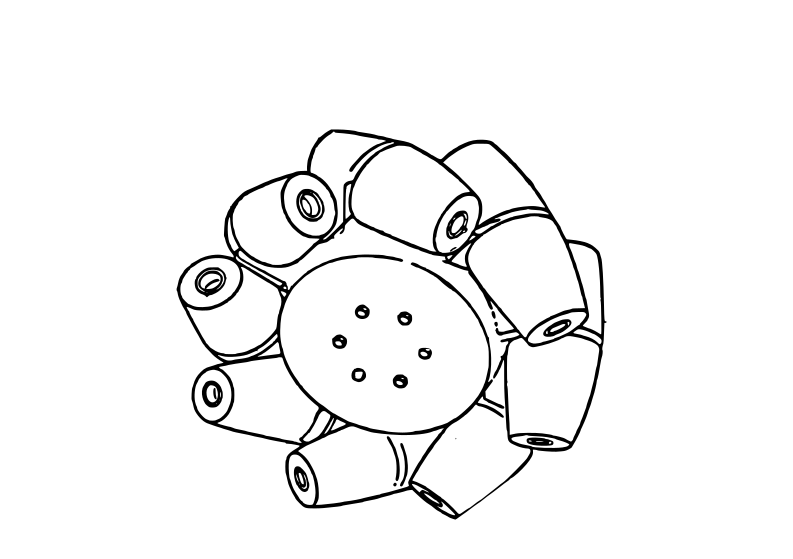
\includegraphics[width=0.4\linewidth]{mecanum_wheel.pdf}
	\caption{Side view of a Mecanum wheel~\cite{Dickerson.1991}}
	\label{fig:mecanumwheel}
\end{figure}
The rollers on a Mecanum wheel are positioned such that their axes are skewed relative to the central wheel axle. This geometry allows each wheel to produce a vector of force that, when combined with the forces generated by the other wheels, results in omnidirectional motion. This configuration avoids the singularities common in traditional wheel systems, which often require significant propulsion adjustments to perform small or intricate maneuvers. Vehicles equipped with Mecanum wheels are therefore able to perform complex maneuvers in confined spaces with greater efficiency, reducing both the time and area required for movement~\cite{Dickerson.1991}.\\
The kinematics of Mecanum wheels also play a crucial role in achieving precise control over a vehicle’s movement. As each wheel operates independently, the control system must convert the desired motion into specific commands for each wheel, accounting for the interaction between longitudinal, lateral, and rotational forces. While this may seem computationally complex, efficient algorithms have been developed to simplify the process. These algorithms, often incorporating compensation for wheel slip, ensure that the vehicle can execute smooth, omnidirectional movement without requiring significant computational overhead~\cite{Dickerson.1991}. In this case a simple control algorithm will be developed that does not use a compensation for wheel slip. As it is a fairly simple and lightweight remote controlled car for studying purposes, the required precision is not so high, that it would justify the increased development effort.\\
One notable disadvantage of the Mecanum wheel design is the inefficient transfer of kinetic energy from the motors to the ground. As the exterior rollers rotate, only a portion of the force generated by the wheels is effectively applied to the ground. This is due to the angled orientation of the rollers, which causes the total force exerted by each wheel to be split into components. Consequently, only a fraction of the force directly contributes to the vehicle’s motion, leading to reduced overall efficiency in propulsion compared to conventional wheels~\cite{F.Adascalitei.2011}.\\
Therefore, Mecanum wheels are not commonly used in applications where efficient energy use is a priority but are favored in scenarios where the efficient use of time and space is essential. Many researchers focus on utilizing these wheels in the design of autonomous vehicles~\cite{Tlale.2008} and robots, particularly for environments where maneuverability is critical. Omni-directional platforms, like those equipped with Mecanum wheels, offer the ability to move instantly in any direction from any position. This provides significant advantages in congested environments filled with static and dynamic obstacles, such as factory workshops, warehouses, hospitals, and elderly care facilities, where conventional wheeled designs would struggle to navigate narrow aisles and tight spaces efficiently~\cite{nivenb.2002}.\\

In this design, four Mecanum wheels are arranged at the four corners of a rectangular vehicle platform, with each wheel oriented to face forward along the X-axis, as can be seen in fig.~\ref{fig:mecanumwheelconfig}. 
\begin{figure}[h]
	\centering
	\captionsetup{justification=centering}
	\includegraphics[width=0.7\linewidth]{mecanum_wheel_configuration.pdf}
	\caption{Wheel configuration and coordinates of Mecanum wheel car~\cite{Dickerson.1991}}
	\label{fig:mecanumwheelconfig}
\end{figure}
The arrangement allows the vehicle to achieve omnidirectional movement, with the X-axis representing forward and backward motion, the Y-axis representing lateral (side-to-side) motion, and the $\theta$ corresponds to rotational (yaw) movement.\\ The control system uses 8-bit signed integers to define motion in each direction, with values ranging from -127 to 127 to ensure symmetry in both positive and negative directions. While 128 would be the theoretical maximum for positive values, it is capped at 127 to maintain balance with the maximum negative value of -127, thus allowing precise and symmetrical control over the vehicle’s motion in all three axes.\\
In order to achieve the desired translational movement of the vehicle along the X and Y axes (see fig.~\ref{fig:mecanumwheelconfig}), each of the four Mecanum wheels must rotate in a specific direction. The table~\ref{tab:mecanumdirection} provides a detailed breakdown of the rotational direction of each wheel corresponding to various translational movements. The wheels, designated as A, B, C, and D in the configuration, can rotate either positively, negatively, or remain idle (0) depending on the intended movement. A positive direction (+) indicates forward rotation, while a negative direction (-) refers to backward rotation. 

\begin{table}[h]
	\centering
	
	\caption{Rotation Direction for Translational Movement~\cite{Tlale.2008}}
	\begin{tabular}{c||c|c|c|c}
		\hline
		Wheel & \textbf{A} & \textbf{B} & \textbf{C} & \textbf{D} \\
		\hline
		\hline
		\textbf{Forward} & + & + & + & + \\
		\hline
		\textbf{Back} & - & - & - & - \\
		\hline
		\textbf{Left} & - & + & + & - \\
		\hline
		\textbf{Right} & + & - & - & + \\
		\hline
		\textbf{Forward-Right} & + & 0 & 0 & + \\
		\hline
		\textbf{Forward-Left} & 0 & + & + & 0 \\
		\hline
		\textbf{Back-Right} & - & 0 & 0 & - \\
		\hline
		\textbf{Back-Left} & 0 & - & - & 0 \\
		\hline
		\textbf{\acs{cw} Turn} & + & - & + & - \\
		\hline
		\textbf{\acs{ccw} Turn} & - & + & - & + \\
		\hline
	\end{tabular}
	\label{tab:mecanumdirection}
\end{table}

The precise coordination of wheel rotations enables the vehicle to move efficiently in any direction, leveraging the omni-directional capability of the Mecanum wheel design.
To translate user input into individual wheel velocities for the Mecanum wheel vehicle, a control scheme is employed that requires three signed integer values. These values correspond to the movement along the X-axis, Y-axis, and the rotational motion ($\theta$). The user provides these three inputs to control the vehicle's motion, which are represented as a 1x3 vector. This vector is then multiplied by a pre-defined translational matrix to convert the input into wheel-specific velocity values for each of the four wheels—designated A, B, C, and D. The resulting output is a 1x4 vector that determines the movement of each wheel individually. The transformation is achieved through the matrix equation~\ref{eq:mecanumtranslation}.

\begin{equation}
	\label{eq:mecanumtranslation}
	\begin{bmatrix}
		x_{val} & y_{val} & \theta_{val}
	\end{bmatrix}
	\cdot
	\begin{bmatrix}
		+1 & +1 & +1 & +1\\
		+1 & -1 & -1 & +1\\
		+1 & -1 & +1 & -1\\
	\end{bmatrix}
	=
	\begin{bmatrix}
		A & B & C & D
	\end{bmatrix}
\end{equation}
The 3x4 matrix represents the relationship between the vehicle's translational and rotational movements and the corresponding velocities of each wheel. The output vector provides the computed speed and direction for each of the four wheels.





	
	\section{Motor Control using PWM}
	\label{sec:TheoryPWM}
	%\todo{Discuss pulse-width modulation (PWM) as a method for motor speed control, with a focus on its advantages over on-off control.}
	
	\section{Wireless Communication Protocols}
	\label{sec:TheoryComm}
	%\todo{Provide a technical description of the communication protocols used for remote control, such as UDP and Bluetooth.}
	
	\subsection{WiFi and UDP}
	
	\subsection{Bluetooth}
	
	\section{Sensor Integration}
	\label{sec:TheorySensors}
	%\todo{Explain the role of sensors in detecting acceleration and orientation for advanced control strategies.}
	
	\chapter{Methodology}
	
	\section{Hardware Selection}
	
	\subsection{Microcontroller (ESP32) | \acs{ej}}
	\label{sub:microESP32}
	%\todo{Discuss the choice of the ESP32 board for its versatility and wireless communication features.}
	The selection of an appropriate microcontroller was a critical aspect of the hardware design for this project. Given the project’s constraints and the need to utilize available components, it was necessary to choose a microcontroller based on readily accessible development boards. After evaluating several options, the ESP32 was identified as the most suitable choice due to its versatile features and broad compatibility with the project’s requirements.\\
The ESP32 microcontroller is a highly versatile and capable device that offers a broad range of features, making it ideal for this project. At its core, the ESP32 incorporates a dual-core, 32-bit Tensilica LX6 microcontroller, based on the Harvard architecture. This architecture separates data and instruction memory, enhancing processing efficiency. The CPU speed is adjustable, ranging from \num{160}~\si{\mega\hertz} to \num{240}~\si{\mega\hertz}, allowing the system to optimize for either performance or energy consumption depending on the operational requirements~\cite{Kareem.2021}. It offers several advantages over other similarly priced microprocessor. Its very low power consumption is particularly beneficial in battery-powered systems like this remote controlled vehicle, extending operational time while minimizing energy drain. Additionally, the ESP32 boasts a high level of integration, including a built-in antenna and step-down converter, simplifying the overall hardware design and reducing the need for additional components~\cite{espressif.07.09.2024}.\\
The ESP32 Dev Kit C is a widely used development board, designed for easy prototyping with the ESP32 microcontroller, it can be seen in fig.~\ref{fig:microprocessor_esp32}. The key components of the board are marked as follows:
\begin{enumerate}
	\item \textbf{Micro USB connector}: Used for powering the board and programming the ESP32 via a USB connection.
	\item \textbf{AMS1117 Voltage regulator}: Ensures the board operates at the required \num{3.3}~\si{\volt} by stepping down input voltage from the Vin pin or the USB connection.
	\item \textbf{CP2102 USB to UART bridge}: Facilitates communication between the USB port and the ESP32, enabling data transfer and debugging.
	\item \textbf{ESP32-WROOM-32 module}: The heart of the board, containing the ESP32 microcontroller.
	\item \textbf{Antenna}: Built-in antenna for wireless communication.
\end{enumerate}
Other notable connections include:
\begin{itemize}
	\item \textbf{GND}: Ground connection used as the negative voltage reference.
	\item \textbf{3V3}: Provides \num{3.3}~\si{\volt} output or requires exactly \num{3.3}~\si{\volt} of input supply voltage for stable operation.
	\item \textbf{Vin}: Can accept a wide input voltage range from \num{4.4}~\si{\volt} to \num{12}~\si{\volt}~\cite{amicu.}, regulated down to \num{3.3}~\si{\volt} internally.
\end{itemize}

\begin{figure}[h]
	\centering
	\captionsetup{justification=centering}
	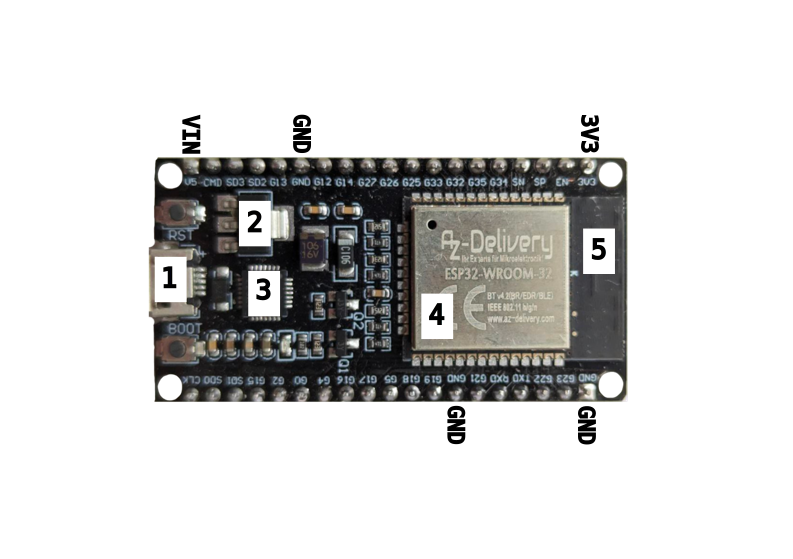
\includegraphics[width=0.6\linewidth]{esp32_board.pdf}
	\caption{ESP32 Dev Kit C Board}
	\label{fig:microprocessor_esp32}
\end{figure}

The ESP32 also boasts an extensive range of input and output (I/O) options. It has 36 \ac{gpio} pins, 18 of which can be used as \ac{adc} inputs, allowing the microcontroller to read sensor data and other analog signals. Furthermore, the ESP32 is equipped with two dedicated \ac{dac} pins, which can generate true analog outputs, a feature that is particularly useful in applications where precise control over analog signals is required. Almost all output-capable pins can also produce \ac{pwm} signals, which are integral to this project for controlling motor speed and direction~\cite{Kareem.2021}.\\
In terms of memory, the ESP32 features both on-chip (internal) and onboard (external) memory. The internal memory is composed of 448 KB of ROM, which is responsible for booting and core functions, and 520 KB of SRAM used for data storage and instructions during runtime. Additionally, the ESP32 supports up to 16 MB of external ISP flash RAM, which can be used to store larger programs or data sets that exceed the capacity of the internal memory~\cite{Kareem.2021}.
One of the ESP32’s most significant features is its built-in communication capabilities. For wireless communication, it supports WiFi with full 802.11 b/g/n/e/i standards. This allows the ESP32 to function as both a client, connecting to a router, and as an access point, creating its own wireless network. This versatility is beneficial for remotely controlling the vehicle via \ac{udp} packets over WiFi. The Bluetooth module supports v4.2 BR/EDR and \ac{ble} standards, with data transfer speeds of up to 4.0~Mbps, making it possible to control the vehicle with Bluetooth devices, such as a \ac{ps4} controller~\cite{Kareem.2021}.\\
In addition to its wireless communication, the ESP32 supports several wired communication protocols, including UART, I2C, ISP, CAN, and I2S. These protocols allow the microcontroller to communicate with a variety of peripheral devices, such as sensors, motor drivers, and other controllers, providing flexibility in system design and integration~\cite{Kareem.2021}.\\
The ESP32 can be programmed using two main frameworks. The first, ESP-IDF, is the official development framework provided by Espressif Systems. It offers low-level access to the hardware and allows developers to take full advantage of the ESP32's dual-core architecture. However, due to its complexity, it is more suited for advanced projects requiring intricate customization. The second framework is the Arduino IDE, which simplifies development by abstracting some of the low-level details~\cite{Kareem.2021}. Although it offers less flexibility in core management compared to ESP-IDF, the Arduino framework provides sufficient functionality for this project and is widely supported with extensive libraries and an open-source community. Given the project's requirements and the ease of development, the Arduino framework was chosen for this application.
	
	\subsection{Power System | \acs{ej}}
	\label{sub:PowerSystem}
	%\todo{Describe the 2S/7.4V LiPo battery setup and the integration of the step-down converter.}
	The power system for the Mecanum wheeled car is designed around two \ac{lipo} batteries connected in series. Each \ac{lipo} cell has a nominal voltage of \num{3.7}~\si{\volt}, resulting in a total voltage of \num{7.4}~\si{\volt} when combined. This configuration provides sufficient voltage to drive the motors and other key components of the car, offering a compact and efficient energy solution for the system. Initially, the plan was to use a dedicated \num{5}~\si{\volt} output step-down converter to supply power to the ESP32 microcontroller. However, this approach was abandoned due to issues arising from the converter's inability to handle the low power requirements of the ESP32 in isolation. The step-down converter was designed for heavier loads, and with only the microcontroller connected, it was operating under a "too light" load condition, causing instability in the power supply.\\
To resolve this, the power system was simplified. The \num{7.4}~\si{\volt} output from the \ac{lipo} batteries became the primary supply voltage for both the motor driver and the ESP32 microcontroller. This configuration is advantageous for two reasons. The motor driver is capable of handling the \num{7.4}~\si{\volt}, which is adequate to power the motors at optimal performance. The ESP32 development board has its own built-in voltage regulator capable of stepping down input voltages as high as \num{12}~\si{\volt} to its required \num{3.3}~\si{\volt} operating voltage. Therefore, the same \num{7.4}~\si{\volt} battery supply could be used to power the ESP32 directly, eliminating the need for an external converter and simplifying the system’s overall design. The ESP32 development board includes a dedicated pin that outputs a regulated \num{3.3}~\si{\volt}, enabling the powering of additional components, such as sensors, that lack their own voltage regulation. This simplifies integration by providing a stable power source for peripherals directly from the microcontroller. This revised power strategy enhances the robustness of the power system while reducing component count and complexity, ensuring reliable operation of both the microcontroller and motors.
	
	\subsection{Motor Driver}
	%\todo{Provide details on the H-Bridge drivers used to control each motor.}
	
	\subsection{Additional Components}
	%\todo{Detail the design and selection of mechanical components like the 3D-printed housing and gamepad for user interaction.}
	
	\section{Software Development}
	
	\subsection{Command Protocol Design | \acs{ej}}
	\label{sub:CommandProtDesign}
	%\todo{Explain the development of a custom command set for car control (e.g., "rc x y z" command).}
	The development of a custom command protocol for controlling the Mecanum wheeled car was essential to ensure smooth and efficient communication between the user and the vehicle. The design is inspired by the \ac{sdk} of the Ryze Tello Drone, which provided a useful framework for structuring commands in a clear and scalable manner~\cite{ryze.2018}. In this system, the Mecanum car operates as a WiFi access point, with a fixed IP address of 192.168.10.1. Devices connecting to the car, such as smartphones or laptops, can communicate through \ac{udp} protocol on specific ports. Commands are sent to UDP port 4444, and status reports are received on UDP port 4445.\\
The command protocol allows for three core commands to be sent to the Mecanum car. These commands, described in the command list, include:
\begin{itemize}
	\item \textbf{rc x y z}: The primary control command that applies speed values to the car's motion. x, y and z are 8-bit signed integer values that correspond to the user input that is translated to the wheels.
	\item \textbf{keepalive}: This command maintains the connection between the client device and the car without issuing any new control instructions. It prevents the system from timing out and maintains the current state of motion until new instructions are given.
	\item \textbf{stop}: This command halts all movement, immediately setting the speeds on all axes to zero, ensuring the car stops regardless of its previous state.
\end{itemize}
Each of these commands is transmitted as a simple string over UDP to ensure minimal latency in communication, and responses such as "ok" or "error" are returned depending on the validity and execution of the command.\\
In addition to receiving commands, the Mecanum car provides real-time feedback via status reports. These reports are sent every second through \ac{udp} port 4445 to the last client device that issued a command. The report is transmitted as a string containing various key data points about the car's current state. This includes:
\begin{itemize}
	\item \textbf{Battery Voltage} (batV): The voltage level of the car’s battery, reported to two decimal places.
	\item \textbf{Battery Percentage (batP)}: The remaining charge of the battery, expressed as a percentage.
	\item \textbf{Motor Duty Cycles} (mA, mB, mC, mD): The current \ac{pwm} duty cycles for each of the four motors (A, B, C, D), expressed in percentage values.
\end{itemize}
This status feedback is critical for maintaining control, as it allows the user to monitor battery levels and motor activity in real time, ensuring effective command execution and enabling adaptive decision-making during vehicle operation.\\
To implement the command protocol, the Mecanum car requires a \ac{udp} client to be set up on the controlling device. The client sends commands to the car and listens for responses on the designated ports. The fixed IP address simplifies the connection process, while the compact command set ensures a minimal overhead for data transmission, making the system both lightweight and responsive. With the foundation of this protocol, the car can be efficiently controlled in real-time, whether for basic movement or more complex, synchronized operations. The whole documentation of Mecanum Car Commands in the style of the Ryze Tello Drone \ac{sdk} can be accessed in the appendix.
	
	\subsection{Python Module | \acs{ej}}
	%\todo{Explain the development of the python module to control the mecanum car.}
	A python module is developed to provide access to control the car using its \ac{sdk} with short and easy commands in Python. The user only has to connect a client, where the Python module is installed, to the car's Wi-Fi \ac{ap}. Each Python command is translated to a string that is sent to the car's IP address and a predefined port. This string is then interpreted by the firmware running on the microcontroller that controls the car. The commands used for steering the car are interpreted as a vector, which is used to control the direction.\\
	
	\subsection{Firmware for ESP32 | \acs{ej}}
	%\todo{Describe the main file and function of the ESP32}
	\lstset{style=customcpp}
The firmware developed for the ESP32 is the core of the Mecanum wheel car's control system, responsible for managing communication protocols, motor control, and system monitoring. The structure of the firmware has been designed to handle different modes of operation, including control via WiFi and Bluetooth, while providing real-time feedback on the car’s status, including battery level monitoring.\\
The firmware begins with the inclusion of essential libraries such as MotorPWM, UDPcontrol, PS4Control, BatteryStatus, and StatusLED. These libraries are integral to the car's operation, providing control over motor speed via PWM, handling the UDP or PS4 control modes, monitoring battery levels, and updating LED indicators for status feedback.\\
The user can choose between two control modes by defining either \lstinline|UDP_CONTROL_MODE| or \lstinline|PS4_CONTROL_MODE|. Only one of these modes should be active at any time, controlling whether the car is operated via WiFi (\acs{udp}) or through a PS4 controller using Bluetooth.
The \lstinline|SERIAL_DEBUG| define can be uncommented to enable serial debugging, which prints relevant system information such as motor speeds and battery levels to the serial monitor. This is useful for development and testing.\\

The \lstinline|setup()| function is responsible for initializing all key components, including the status LED, playing the startup animation indicating successful booting, and to start the communication processes. At the end of the startup process the battery value is checked once to store it in memory. Additionally memory space is reserved for the motor control arrays where the control input from the user is and the \ac{pwm} values for motors are stored. The whole process can be seen in fig.~\ref{fig:SetuopSequence}.

\begin{figure}[h]
	\centering
	\captionsetup{justification=centering}
	\includegraphics[width=1\linewidth]{Boot_Sequence_WiFiAP.pdf}
	\caption{Setup Sequence of Microprocessor}
	\label{fig:SetuopSequence}
\end{figure}

Afterwards the main \lstinline|loop()| function is entered, which loops infinitely. This function continuously checks for control input by the user and updates the motor outputs. 

 This function is the main execution loop that continuously checks for control input (either from UDP packets or PS4 controller), calculates motor speeds, and updates the motor outputs. It also checks the battery status every second and sends status messages back to the controller in UDP mode. At the same time this function checks the battery status periodically and sends the status message back to the user after a specified time interval passes. This process can be seen in fig.~\ref{fig:MainLoopSequence}.

\begin{figure}[h]
	\centering
	\captionsetup{justification=centering}
	\includegraphics[width=1\linewidth]{LoopSequence_WiFiAP.pdf}
	\caption{Main Loop Sequence of Microprocessor}
	\label{fig:MainLoopSequence}
\end{figure}

The firmware for the ESP32 microcontroller plays a crucial role in the operation of the Mecanum wheel car. It efficiently manages the control modes, motor control, and system monitoring while providing flexibility in terms of communication protocols (WiFi/UDP or Bluetooth). The modularity of the firmware allows for future extensions and adjustments as needed for enhanced functionality or new features. For example new sensors can be added which are checked at the same time as the battery level. The status message can also be expanded to accustom for more sensor data that needs to be transmitted.
	
	\subsection{Motor Control Algorithm}
	%\todo{Describe how steering commands are translated into PWM signals to adjust motor speed.}
	
	\subsection{Sensor Integration}
	%\todo{Discuss the integration of the 6-DoF sensor for advanced control, if implemented.}
	
	\subsection{Android App | \acs{ej}}
	\label{sub:AndroidApp}
	%\todo{Explain the development of the Android App}
	The Android application used to control the Mecanum wheel car was developed in Kotlin and built using Android Studio. The primary motivation behind creating the app was to offer a smartphone-based control system for the car via WiFi, using UDP packets for communication. This system offers a simple interface for directional movement, speed control, and vehicle status feedback, all integrated into an intuitive layout designed for ease of use, which can be seen in fig.~\ref{fig:AppScreenshot}.

\begin{figure}[h]
	\centering
	\captionsetup{justification=centering}
	\includegraphics[width=0.3\linewidth]{App_Screenshot.jpg}
	\caption{Screenshot from the Android App}
	\label{fig:AppScreenshot}
\end{figure}

The app allows users to control the car by sending directional commands to move the car in one of eight base directions—up, down, left, right, and the diagonals—using on-screen buttons. Additionally, users can rotate the car clockwise or counterclockwise using designated buttons. The interface ensures that each directional button initiates movement when pressed and sends a "stop" command as soon as the button is released. If a button is pressed for longer than 8 seconds, the app sends a "keepalive" message, ensuring the car does not time out due to inactivity.
At the bottom of the screen, a slider allows the user to adjust the speed of the car dynamically, ranging from slow to fast movement. The speed value is converted into control commands that are transmitted via UDP to the car.\\
The layout of the app consists of three key areas:
\begin{itemize}
	\item \textbf{Directional Buttons}: These are located centrally on the screen and allow users to control the car's movement. Each button corresponds to one of the eight base directions or rotation commands (clockwise and counterclockwise).
	\item \textbf{Speed Control Slider}: Positioned at the bottom, this slider allows users to adjust the car's speed. The value is continuously read and used to form the movement command strings sent over UDP.
	\item \textbf{Status Area}: The top of the app displays a battery symbol, which is updated with real-time information about the car’s battery status and motor activity, based on UDP status messages sent by the car.
\end{itemize}

To control the car, the app transmits UDP packets to the Mecanum car, which is set to the IP address "192.168.10.1" on port 4444. A mapping function inside the app converts button presses into the respective command strings in the format "rc x y z". Here, x and y represent the speed in the respective direction, and z indicates rotation speed. The app ensures that each command reflects the user's intended movement, and every release of a button triggers a "stop" command to halt the car.
The app makes use of the keepalive-mechanism, which is automatically triggered if a button is held down for more than 8 seconds. The app sends this message to prevent the car from entering a timeout state during continuous use. The keepalive packet is sent periodically to maintain the connection and avoid interruptions in operation.\\
In addition to sending movement commands, the app listens for status updates from the car on UDP port 4445. These updates contain vital information about the car’s battery voltage and motor performance, which are displayed in the status area at the top of the screen. The data is presented clearly for the user, with battery voltage and percentage shown next to a battery icon, while individual motor performance is displayed in terms of percentage. The app’s interface also includes a battery status checker, which updates in real time based on incoming messages from the car. This ensures that the user can monitor the car’s battery condition and make informed decisions about operational time.\\
Though the current version of the app provides a reliable interface for controlling the Mecanum car, future iterations could integrate additional features such as customizable control schemes or enhanced feedback, such as warnings when the battery is low.
This Kotlin-based application forms a robust foundation for further development, ensuring that users can control the car seamlessly over WiFi, with real-time status monitoring and intuitive controls.
	
	\section{Communication Interface}
	
	\subsection{WiFi/UDP Control System}
	%\todo{Describe how commands are transmitted using UDP packets.}
	
	\subsection{Bluetooth Integration with PS4 Controller}
	%\todo{Detail the steps to integrate Bluetooth communication with a PS4 controller.}
	
	\chapter{Results and Discussion}
	
	\section{Hardware Assembly}
	%\todo{Discuss the success of the hardware selection and assembly, highlighting any issues encountered during wiring or housing assembly.}
	
	\section{Software Performance}
	%\todo{Analyze the performance of the motor control algorithm and the responsiveness of the control system via WiFi or Bluetooth.}
	
	\section{Sensor Data and System Feedback}
	%\todo{If implemented, discuss the results of using the 6-DoF sensor for detecting acceleration and its effect on control precision.}
	
	\section{Challenges and Limitations}
	%\todo{Identify any challenges faced during development (e.g., limitations in hardware or communication delays) and how they were mitigated.}
	
	\chapter{Conclusion}
	\label{ch:Conclusion}
	%\todo{Summary of Achievements: Summarize the key outcomes of the project, such as the successful development of PWM-based motor control and wireless steering}
	
	%\todo{Future Work: Propose potential future enhancements, such as improving the sensor-based control or refining the 3D-printed housing design}
	
	%\todo{Final Remarks: Reflect on the broader implications of the project and its contribution to the field of robotics or vehicle control systems.}
	
	\chapter*{List of Acronyms}
	\label{sec:Acro}
	\begin{acronym}[SDK]
		\acro{adc}[ADC]{analog-to-digital converter}
		\acro{ap}[AP]{Access Point}
		\acro{ble}[BLW]{Bluetooth Low-Energy}
		\acro{cw}[CW]{clockwise}
		\acro{ccw}[CCW]{counterclockwise}
		\acro{dac}[DAC]{digital-to-analog converter}
		\acro{dof}[DoF]{Degrees of Freedom}
		\acro{gpio}[GPIO]{general-purpose input/output}
		\acro{lipo}[LiPo]{lithium polymer}
		\acro{ps4}[PS4]{Sony Playstation 4}
		\acro{pwm}[PWM]{pulse-width modulation}
		\acro{sdk}[SDK]{Software Development Kit}
		\acro{udp}[UDP]{User Datagram Protocol}
		\acro{ac}[AC]{Anil Chhotala}
		\acro{ak}[AK]{Axit Kakadiya}
		\acro{ds}[DS]{Devraj Solanki}
		\acro{ej}[EJ]{Edmund Jochim}
	\end{acronym}
	
	\clearpage
	\pagenumbering{Roman}
	\setcounter{page}{5}
	
	\chapter*{Appendix}
	
	{\Large \textbf{Mecanum Car Commands}}\\
	Use Wi-Fi to establish a connection between the Mecanum Car and a client device.\\
	\begin{tcolorbox}[width=\linewidth, sharp corners=all, colback=white!95!black, boxrule=0pt]
		{\large \textbf{Send Command \& Receive Response}}
	\end{tcolorbox}
	Mecanum Car IP: \textbf{192.168.10.1} UDP Command Port: \textbf{4444} UDP Status Port: \textbf{4445}
	
	\begin{tabular}{R{0.1\textwidth} L{0.85\textwidth}}
		Step 1:\newline \phantom{-} & Set up a UDP client on the client device to send and receive messages from the Mecanum Car via the same port. \\
		Step 2:\newline \phantom{-} & Send any available command to the Mecanum Car to control it. \\
	\end{tabular}
	
	\begin{tcolorbox}[width=\linewidth, sharp corners=all, colback=white!95!black, boxrule=0pt]
		{\large \textbf{Control Commands}}
	\end{tcolorbox}
	\begin{tabularx}{\textwidth}{c|c|c}
		\hline
		\textbf{Command} & \textbf{Description} & \textbf{Possible Response} \\
		\hline
		rc x y z & \makecell{Apply speed to  x y or z direction.\\x (backward - forward) = -127 to 127\\y (left - right) = -127 to 127\\z (rotation ccw - cw) = -127 to 127} & -/error \\
		\hline
		keepalive & \makecell{Keeps connection to Mecanum Car alive.\\Prevents timeout without changing last command.} & ok/error \\
		\hline
		stop & \makecell{Set all directions to 0.} & ok/error \\
		\hline
	\end{tabularx}
	\\
	\begin{tcolorbox}[width=\linewidth, sharp corners=all, colback=white!95!black, boxrule=0pt]
		{\large \textbf{Status Message | Data Type: String}}
	\end{tcolorbox}
	\textbf{Data string received every second while controlling via WiFi}\\
	"batV:\%.2f,batP:\%d,mA:\%d,mB:\%d,mC:\%d,mD:\%d,:\textbackslash n"\\
	\\
	\textbf{Description}\\
	"batV" = Measured voltage of battery in Volt\\
	"batP" = Charge of battery in Percent\\
	"mX" = Duty cycle of motor X in Percent\\

	
	\bibliography{lit_master}
	
\end{document}